\documentclass[11pt]{article}

\usepackage[margin=1in]{geometry}
\usepackage{tikz}
\usepackage{mathtools}
\DeclarePairedDelimiter\ceil{\lceil}{\rceil}
\DeclarePairedDelimiter\floor{\lfloor}{\rfloor}

\date{}

\begin{document}

\begin{center}
\noindent{\bf {\LARGE COMP 3804: Assignment 3}}\\
Fall  2022\\

\end{center}
\noindent School of Computer Science\hfill{Carleton University}

\noindent \hrulefill

\vspace{5pt}
\noindent
{\bf Due Date: Sunday, November $ 20^{th}$ at 11:59PM}\\

**********  Note that we extended the deadline for this assigment to the  21st **********\\

\noindent
Your assignment should be submitted online on Brightspace as a single PDF file; the filename includes your studentID. No late assignments will be accepted. You can type your assignment or you can upload a scanned copy of it. Please use a good image capturing device. Make sure that your upload is clearly readable. If it is difficult to read, it will not be graded!




%%%%%%%%%%%% NEW SECTION %%%%%%%%%%%%%%%%%
\section*{Question 1 [20 marks]}
Show how Bellman-Ford's and Dijkstra's algorithms would compute the shortest paths from $A$ to all vertices of the graph shown in Figure~\ref{fig:SP}. Illustrate the algorithms as shown in class:  Bellman-Ford via a sequence of graphs (see slide 22). Dijkstra's (see slide 36) by filling in a table with step numbers as row index, vertices as column index, and d[], π[] values as entries. Circle a d[]-value when it is finalized, i.e., when it become δ[] .

\begin{figure}[!ht]
\centerline{\resizebox{!}{0.35\textwidth}{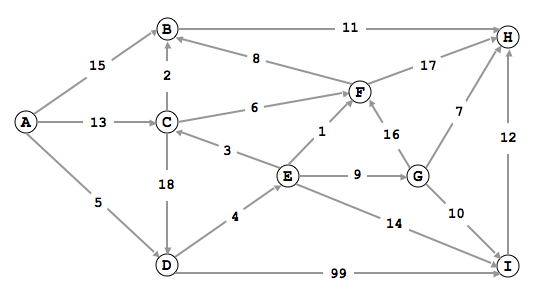
\includegraphics{iu.png}}}
\caption{The input graph for Question 1.}
\label{fig:SP}
\end{figure}



%%%%%%%%%%%% NEW SECTION %%%%%%%%%%%%%%%%%
\section*{Question 2 [20 marks]}
Assume that we are given an undirected graph G=(V,E).  Consider that Dijkstra's algorithm found a shortest path in G, called SP,  between two nodes A and X of V. Is it true or false that if we reverse the nodes on SP, we get a shortest path from X to A? Prove or disprove. 



%%%%%%%%%%%% NEW SECTION %%%%%%%%%%%%%%%%%
\section*{Question 3 [10 marks]}

\begin{enumerate}
	\item
List three different topological orderings for the enclosed graph.
\item Draw a (connected, directed) graph for which no topological sorting order exists.
\end{enumerate}
	
	
\begin{figure}[!ht]
	\centerline{\resizebox{!}{0.75\textwidth}{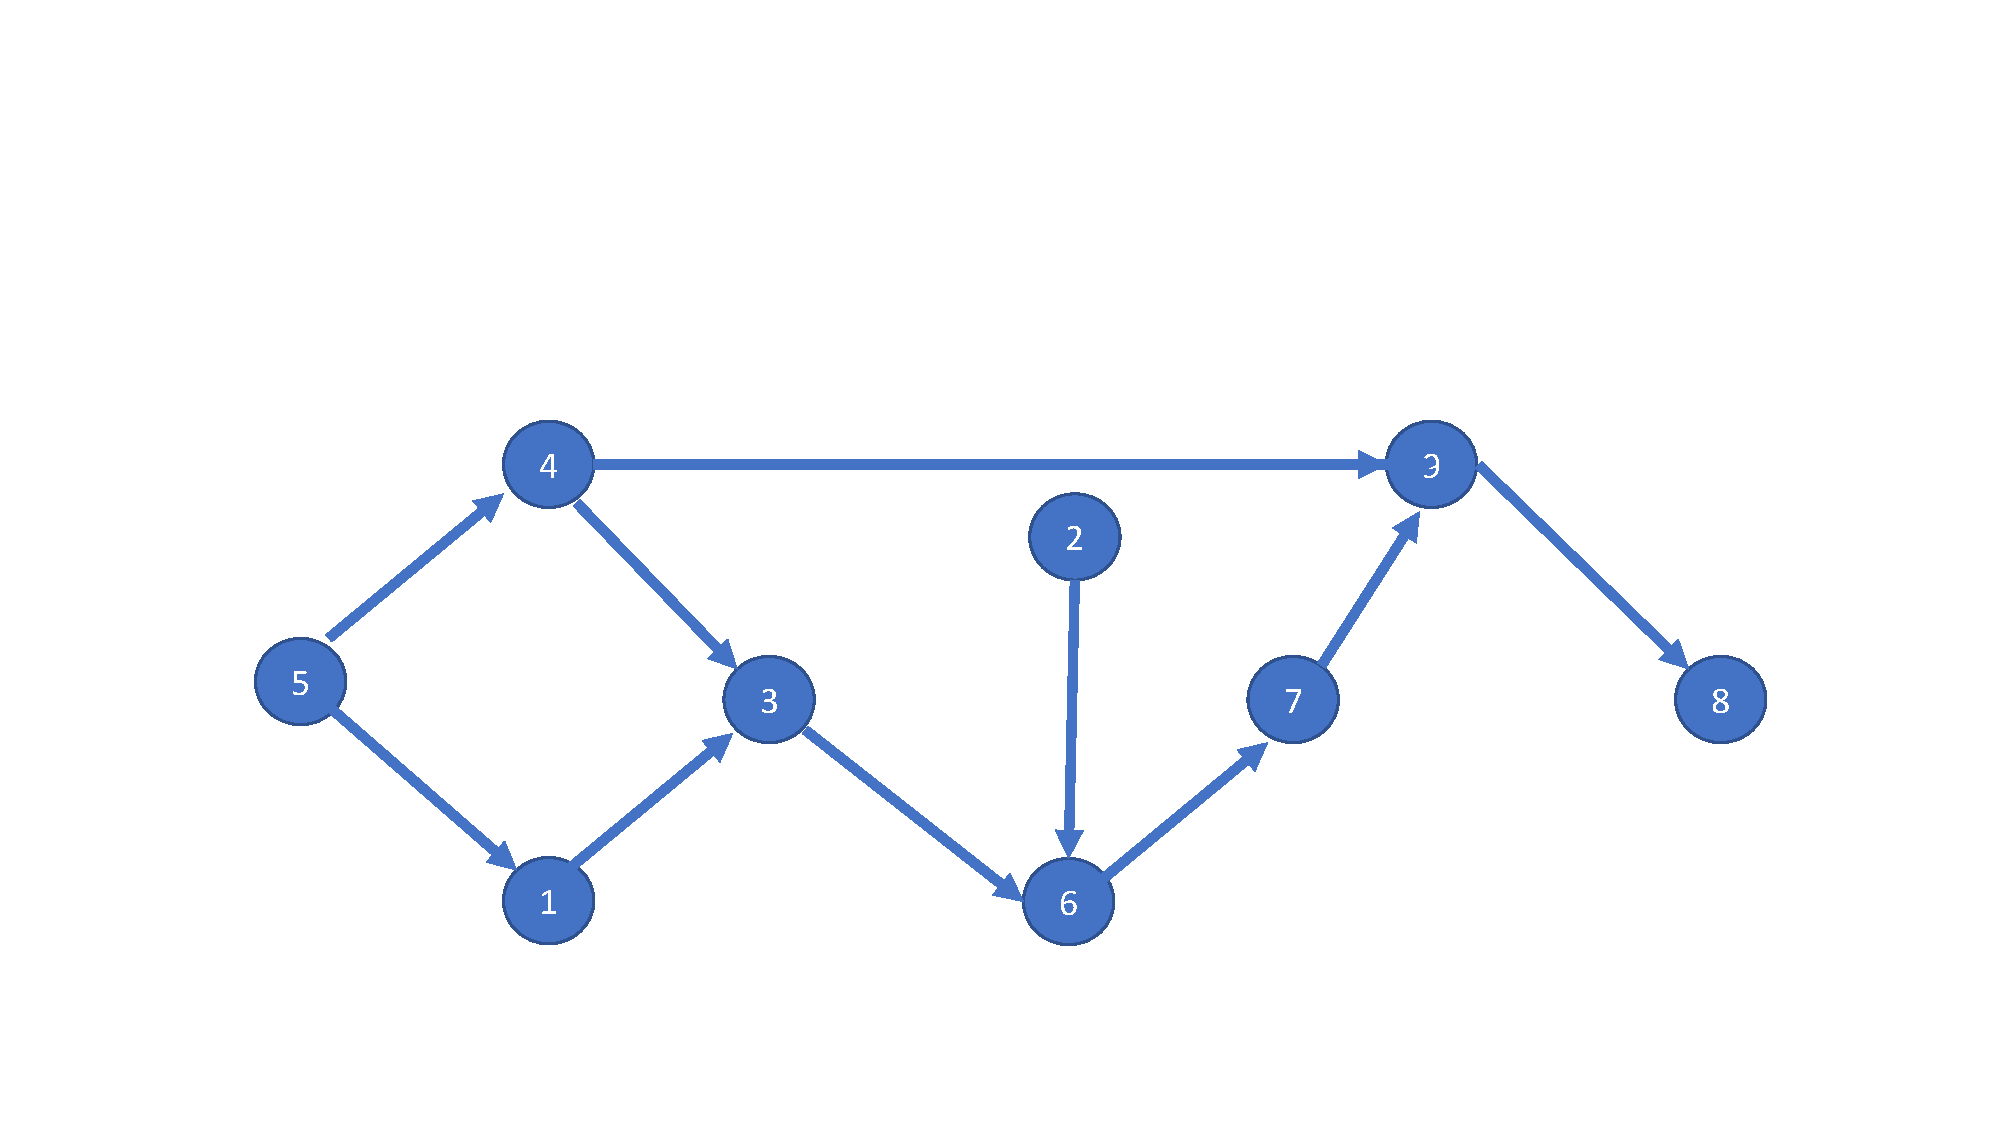
\includegraphics{toposort.pdf}}}
	\caption{The input graph for Question 3.}
	\label{fig:SP}
\end{figure}

%%%%%%%%%%%% NEW SECTION %%%%%%%%%%%%%%%%%
\section*{Question 4 [10 marks]}
Can Dijkstra's algorithm be used to determine if a graph is connected? How does that compare to algorithms for graph connectivity that you may know from previous classes or that you read up (and cite)? Just list the algorithm used and compare the time complexity.



%%%%%%%%%%%% NEW SECTION %%%%%%%%%%%%%%%%%
\section*{Question 5 [10 marks]}
We said that the input to PRIM’s algorithm is a connected, undirected graph. Suppose by accident, we give an input graph that is not connected. What would happen?

%%%%%%%%%%%% NEW SECTION %%%%%%%%%%%%%%%%%
\section*{Question 6 [12 marks]}

Suppose that we are considering a directed, acyclic graph G. A  $Hamiltonian \ path$ is a path in G that visits each vertex of G exactly once. Considering the below four statements, when  does  topological sorting of  G yield a unique solution? Draw a counter-example and argue for each of the four statements  in case it is incorrect below is incorrect and prove  its correctness, otherwise.

\begin{enumerate}
	\item When a single vertex exists in G with  indegree 0.
	\item When several vertices have indegree 0.
	\item When a single vertex exists in G with  outdegree 0.
	\item When there  exists a Hamiltonian path in G.
	
	
\end{enumerate}

\begin{center}
	\noindent{\bf End of Assignment 3.}
\end{center}

\end{document}